\chapter{Multi-task learning}

So far we have considered \ac{AES} and \ac{NLI} as independent tasks and
performed experiments on both tasks separately. We will now try to train
models to predict both tasks simultaneously.


\section{Models}

We selected four models for the multi-task experiments, two convolutional and
two recurrent neural networks. They were chosen based on the macro \FI results
on the development set. The two \acp{CNN} chosen were the two \acp{CNN} that
had the highest macro \FI on the full set of labels in the development set,
and likewise for the two \acp{RNN}.

\begin{table}
  \centering
  \begin{tabular}{lll}
    \toprule
    Hyperparameter & CNN1 & CNN2 \\
    \midrule
    Embedding size & \multicolumn{2}{c}{100} \\
    $L_2$ constraint & \multicolumn{2}{c}{3} \\
    Embedding init & Random & Pre-trained \\
    Input representation & Mixed UPOS & Tokens \\
    \bottomrule
  \end{tabular}
  \caption{Descriptions of the two CNN models}
  \label{tab:cnn-parameters}
\end{table}

\begin{table}
  \centering
  \begin{tabular}{lll}
    \toprule
    Hyperparameter & RNN1 & RNN2 \\
    \midrule
    Word embeddings & \multicolumn{2}{c}{Dynamic} \\
    Embedding size & \multicolumn{2}{c}{100} \\
    RNN cell & \multicolumn{2}{c}{GRU} \\
    Pooling method & \multicolumn{2}{c}{Attention} \\
    Bidirectional & \multicolumn{2}{c}{Yes} \\
    Embedding init & Random & Pre-trained \\
    Input representation & Tokens+UPOS & Tokens \\
    \bottomrule
  \end{tabular}
  \caption{Descriptions of the two RNN models}
  \label{tab:rnn-parameters}
\end{table}

In order to learn more about the variance of results, we trained each model
five times for each auxiliary loss weight with five different random seeds.


\section{Results}

In table \ref{tab:multitask-results}, we see the results of running some of
the most successful models from the previous chapter in a multi-task setting,
using the essay's L1 as the auxiliary label to predict. The number following
the model name is the weight given to the auxiliary loss during training.
Each model is listed with an associated number which is the weight given to
the auxiliary task in training. The number 0 indicates a single-task setup,
and 0.5 indicates equal weight given to both tasks in training.

The reported metrics apply to the main task, CEFR prediction, only. It seems
that the auxiliary task is beneficial for all CNN models. All CNN models get
higher macro and micro \FI in the multi-task setup. Moreover, a higher weight
given to the auxiliary L1 prediction task seems to improve macro \FI
performance across the board. The effect of the auxiliary task weight seems
less clear on the micro \FI, but remember that in our setup, the micro \FI is
a side effect of the highest macro \FI seen during training.

\todo{new models}
\todo{graph effect of loss weight on metrics}

\begin{table}
  \centering
  \begin{tabular}{lrrrr}
    \toprule
            & \multicolumn{2}{c}{All labels}       & \multicolumn{2}{c}{Collapsed labels} \\
    \cmidrule(lr){2-3}
    \cmidrule(lr){4-5}
    Model     & Macro \FI        & Micro \FI        & Macro \FI        & Micro \FI \\
    \midrule
    % $BEGIN autotable multitask-results
    % $META models-per-row=2 columns-per-model=macrof1,microf1
    % $ROW CNN1 0:      cnn-26094553_05          cnn-26094553_06
    % $ROW CNN1 0.25:   cnn-multi-26199963_1     cnn-multi-26199963_2
    % $ROW CNN1 0.5 :   cnn-multi-26199963_3     cnn-multi-26199963_4
    % $ROW CNN1 0.75:   cnn-multi-26199963_5     cnn-multi-26199963_6
    % \midrule
    % $ROW CNN2 0:      cnn-26094553_11          cnn-26094553_12
    % $ROW CNN2 0.25:   cnn-multi-26199963_7     cnn-multi-26199963_8
    % $ROW CNN2 0.5 :   cnn-multi-26199963_9     cnn-multi-26199963_10
    % $ROW CNN2 0.75:   cnn-multi-26199963_11    cnn-multi-26199963_12
    % \midrule
    % $ROW RNN1 0:      rnn-25858209             rnn-25858211
    % $ROW RNN1 0.25:   rnn-multi-26199963_13    rnn-multi-26199963_14
    % $ROW RNN1 0.5 :   rnn-multi-26199963_15    rnn-multi-26199963_16
    % $ROW RNN1 0.75:   rnn-multi-26199963_17    rnn-multi-26199963_18
    % \midrule
    % $ROW RNN2 0:      rnn-25985451             rnn-25985452
    % $ROW RNN2 0.25:   rnn-multi-26199963_19    rnn-multi-26199963_20
    % $ROW RNN2 0.5 :   rnn-multi-26199963_21    rnn-multi-26199963_22
    % $ROW RNN2 0.75:   rnn-multi-26199963_23    rnn-multi-26199963_24
    % $END autotable
    CNN1 0 & $0.235$ & $0.382$ & $0.404$ & $0.699$ \\
    CNN1 0.25 & $0.233$ & $0.439$ & $0.380$ & $0.715$ \\
    CNN1 0.5 & $0.246$ & $0.398$ & $0.389$ & $0.732$ \\
    CNN1 0.75 & $0.247$ & $0.431$ & $0.408$ & $0.707$ \\
    \midrule
    CNN2 0 & $0.255$ & $0.447$ & $0.393$ & $0.740$ \\
    CNN2 0.25 & $0.259$ & $0.455$ & $0.406$ & $0.764$ \\
    CNN2 0.5 & $0.270$ & $0.415$ & $0.398$ & $0.748$ \\
    CNN2 0.75 & $0.275$ & $0.463$ & $0.414$ & $0.780$ \\
    \midrule
    RNN1 0 & $\mathbf{0.354}$ & $0.390$ & $0.493$ & $0.724$ \\
    RNN1 0.25 & $0.301$ & $0.431$ & $0.506$ & $0.797$ \\
    RNN1 0.5 & $0.333$ & $0.472$ & $0.529$ & $0.772$ \\
    RNN1 0.75 & $0.283$ & $\mathbf{0.488}$ & $0.526$ & $0.772$ \\
    \midrule
    RNN2 0 & $0.277$ & $0.407$ & $\mathbf{0.624}$ & $0.756$ \\
    RNN2 0.25 & $0.320$ & $0.423$ & $0.565$ & $0.683$ \\
    RNN2 0.5 & $0.292$ & $0.447$ & $0.533$ & $0.772$ \\
    RNN2 0.75 & $0.285$ & $0.447$ & $0.428$ & $\mathbf{0.805}$ \\
    \bottomrule
  \end{tabular}
  \caption{CNN1: Static, pre-trained embeddings size 50.
           CNN2: Static, pre-trained embeddings size 50, POS as side input.
           RNN1: Attention model with GRU cell, dynamic pre-trained
           embeddings size 50.
           RNN2: Attention model with LSTM cell, dynamic pre-trained
           embeddings size 50, POS as side input.}
  \label{tab:multitask-results}
\end{table}


\todo{do this}
Something with the confidence intervals


For the RNNs, the results are not quite as clear. The multi-task models were
not able to exceed the macro \FI scores of $0.354$ (all labels) and $0.624$
(collapsed labels), but this may be because the macro \FI metric is unstable
because of the `A2' class with one single example in the dev set. For the
same models, accuracy did increase in the multi-task setup.

The model `RNN1 0.5' was the best performing multi-task model by several
metrics. In addition to macro \FI, it was the best in terms of RMSE
($0.888$), MAE ($0.610$), Pearson's correlation coefficient ($0.765$) and
Spearman's ranked correlation coefficient ($0.768$).


\begin{figure}
  % cnn-multi-26199963_11
  \begin{subfigure}{\linewidth}
    \centering
    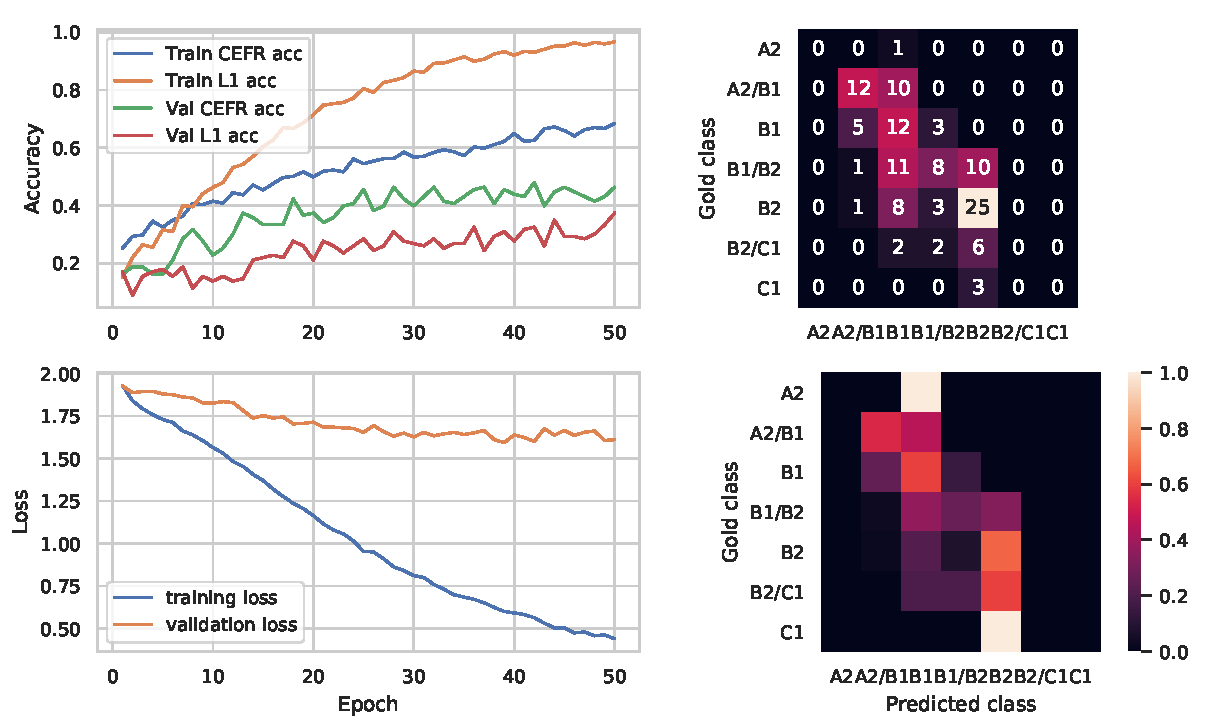
\includegraphics{cnn-multi-training}
    \caption{Training and validation loss and accuracy over 50 epochs of training.}
  \end{subfigure}
  \begin{subfigure}{\linewidth}
    \centering
    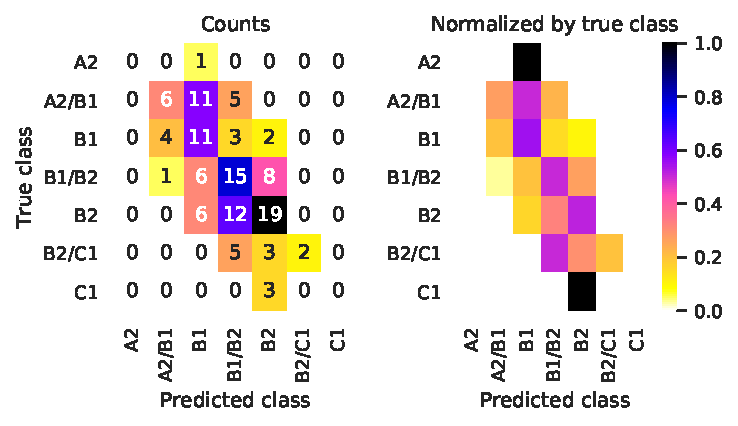
\includegraphics{cnn-multi-confusion}
    \caption{Confusion matrix on validation set, raw counts and normalized.}
  \end{subfigure}
  \caption{CNN2 0.75}
  \label{fig:cnn-multi-training}
\end{figure}

\begin{figure}
  % rnn-multi-26199963_15
  \begin{subfigure}{\linewidth}
    \centering
    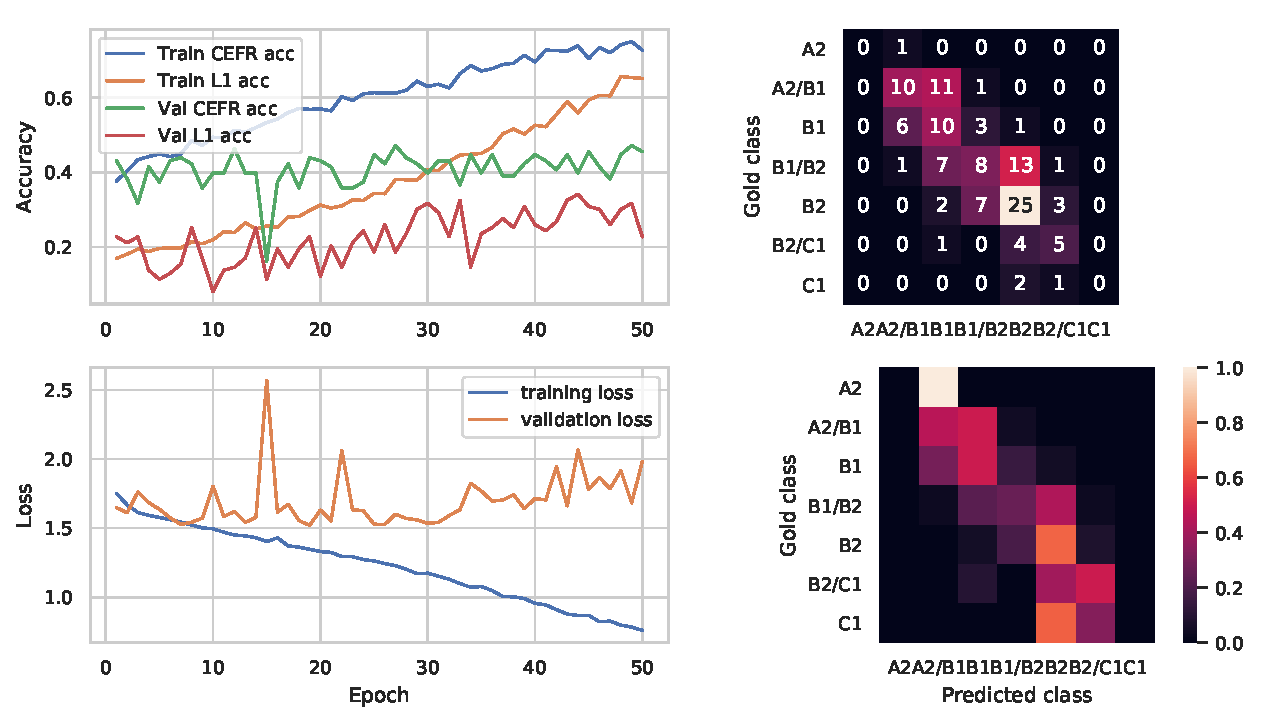
\includegraphics{rnn-multi-training}
    \caption{Training and validation loss and accuracy over 50 epochs of training.}
  \end{subfigure}
  \begin{subfigure}{\linewidth}
    \centering
    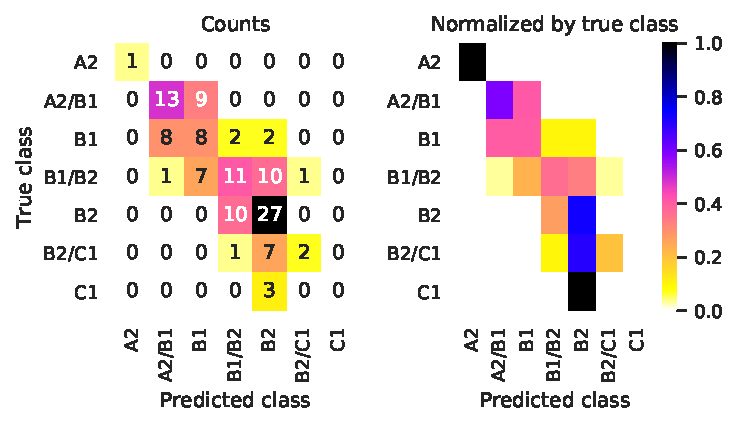
\includegraphics{rnn-multi-confusion}
    \caption{Confusion matrix on validation set, raw counts and normalized.}
  \end{subfigure}
  \caption{RNN1 0.5}
  \label{fig:rnn-multi-training}
\end{figure}


\section{Stability}

By training the model several times with different random seeds, we can see
how much the final results vary. Running a single model ten times with
different random seed gave macro \FI scores in the range from $0.268$ to
$0.341$. The variance of results makes it impossible to conclude which model
is actually the best, as long as we only have the results from a single
training and evaluation run. By running each experiment many times, we could
get a more robust estimate of the true expected performance of the model.


\section{Correlation of metrics}

We have previously discussed different evaluation metrics. Since we now have
trained and evaluated a number of different models, it is possible to see whether
the metrics agree on the ranking of models.

Macro \FI and macro \ac{MAE} correlates only weakly, as seen in figure
\ref{fig:f1-vs-mae}, but they seem to agree on the highest ranking models:
The Pareto front consists of only two samples. The samples in the plot are
models that predict the full seven classes.

\begin{figure}
  \centering
  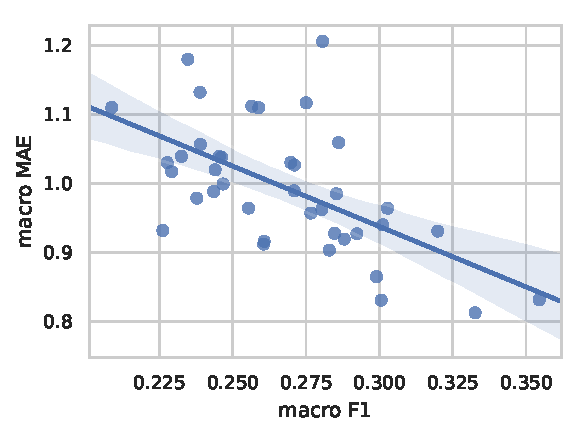
\includegraphics{f1-vs-mae}
  \caption[Macro \FI versus macro MAE]{
    Macro \FI versus macro MAE. Pearson's correlation coefficient = $-0.5945$,
    $p < 10^{-4}$. The shaded area covers a 95\% confidence interval for the
    line of regression.
  }
  \label{fig:f1-vs-mae}
\end{figure}
